%%%%%
%%Title: HiPi+Bus V0.1 Chapter 2 sec 3
%%Creator: Ando Ki
%%CreationDate: April 1992
%%FileName: sec3
%%RelatedFile: ch2
%%%%%
\section{중재 방법}
\subsection{선형 자가 중재 기법}
선형 자가 중재 기법(linear self arbitration scheme : LSAS)의 특징은
중재에 참가하는 각 중재기에 개별적인 중재 요청선을 할당하며,
이들 요청선들의 집합이 중재 버스를 형성하고,
중재 동작이 각 중재기에서 동일하게 수행되어 스스로 중재를 수행한다는 것이다.
이때 중재의 결과는 우선순위에 의해 결정된다. \\
{\tt <}그림~\ref{figure:arbiter}{\tt >}에 선형 자가 중재 기법에
기초한 중재기(arbiter)의 일례를 나타내었다.
\begin{figure}[htb]
   \centerline{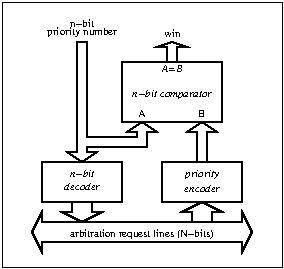
\includegraphics{ch2/FIG/arbiter.jpg}} %\centerline{\psfig{figure=ch2/FIG/arbiter.ps}}
   \caption{선형 자가 중재기의 일례}\label{figure:arbiter}
\end{figure}
중재는 버스 클럭을 기본단위로 하여 이루어진다. 즉 매 버스 클럭마다 한번의 중재가 이루어진다.
각 중재기에는 n-비트 우선순위(priority number)가 할당된다.
n-to-1 멀티플렉서(multiplexer)는 n-비트 우선순위 값을 입력으로 받아
이를 디코딩(decoding)하여
N-비트 폭의 신호선들 중 특정한 하나의 신호선을 구동한다.
이때 n과 N은 $n = \lceil \log_{2} N \rceil$\footnote{$\lceil x \rceil$ :
denotes the least integer that is greater than or equal to x.}의 관계에 있다.
우선순위 엔코더(priority encoder)는 N-비트 중재신호를 입력으로 받아
이들 중 가장 높은 우선순위를 갖는 신호의 번호를 엔코딩하여 출력한다.
비교기(comparator)는 미리 할당된 중재번호와 우선순위 엔코더에서 출력된 값을
비교하여 이들 둘이 같은지 여부를 출력한다.
따라서 비교기에서 출력이 있으면 해당 중재기가 현재 진행 중인 중재동작에서 가장 우선순위가
높은 것이므로 중재에서 이긴 것이 된다.
%
\subsection{공정성 규칙}
선형 자가 중재 방법은 기본적으로 우선 순위에 기초한 것이므로
우선순위가 높은 중재기가 상대적으로 자주 중재에서 이길 것이므로 균등한 중재 결과를 보장하기는 어렵다.
이러한 문제를 해결하기 위해서 가능한 균등하게 사용 기회를 제공하도록 하는 공정성 규칙(fairness rule)을
고려한다. \\
{\tt <}그림~\ref{figure:fairness}{\tt >}에 공정성 규칙을 나타내었다.
%\begin{figure}[htb]
%   \centerline{\psfig{figure=ch2/FIG/fairness.ps}}
%   \caption{공정성 중재 규칙}\label{figure:fairness}
%\end{figure}
%%%%%
%%Title: HiPi+Bus V0.2 Chapter 2
%%Creator: Ando Ki
%%CreationDate: April 1992
%%FileName: ch2
%%RelatedFile:
%%%%%
%\documentstyle[11pt,doublespace,a4wide,psfig]{hbook}
%\setstretch{1.2}
%\begin{document}
%
\begin{figure}[htb]
\begin{center}
  \begin{picture}(240,257)(-120,-257)
	\thicklines
	\put(0,-25){\circle{20}}
	\put(-45,-100){\framebox(90,45){}}
		\put(0,-70){\makebox(0,0){구동되어 있는}}
		\put(0,-82){\makebox(0,0){중재요청신호의}}
		\put(0,-94){\makebox(0,0){수를 계산한다}}
	\put(0,-120){\line(-5,-2){45}}
	\put(0,-120){\line(5,-2){45}}
	\put(0,-156){\line(-5,2){45}}
	\put(0,-156){\line(5,2){45}}
		\put(0,-138){\makebox(0,0){0 또는 1 ?}}
	\put(-91,-202){\framebox(72,36){}}
		\put(-55,-181){\makebox(0,0){다음 중재 싸이클}}
		\put(-55,-193){\makebox(0,0){까지 기다린다}}
	\put(19,-202){\framebox(72,36){}}
		\put(55,-181){\makebox(0,0){중재를}}
		\put(55,-193){\makebox(0,0){수행한다}}
	\put(55,-232){\circle{20}}
	\put(0,-35){\vector(0,-1){20}}
	\put(0,-100){\vector(0,-1){20}}
	\put(-45,-138){\line(-1,0){10}} \put(-55,-138){\vector(0,-1){28}}
		\put(-47,-136){\makebox(0,0)[rb]{아니오}}
	\put(45,-138){\line(1,0){10}} \put(55,-138){\vector(0,-1){28}}
		\put(47,-136){\makebox(0,0)[lb]{예}}
	\put(55,-202){\vector(0,-1){20}}
	\put(-45,-202){\line(0,-1){10}} \put(-45,-212){\line(-1,0){56}}
		\put(-101,-212){\line(0,1){167}} \put(-101,-45){\vector(1,0){101}}
	\put(-120,-257){\framebox(240,257){}} % 외곽 box
  \end{picture}
\end{center}
  \caption{공정성 중재 규칙}\label{figure:fairness}
\end{figure}
%%%%
%\end{document}
%%%%

중재가 버스 클럭을 기본단위로 이루어지므로 공정성 규칙도 버스 클럭 단위로 이루어진다.
중재에 참가하기에 앞서 현재 중재에 참가하고 있는 중재기의 갯수를 파악한다.
이것은 중재 버스에 현재 구동되어 있는 중재 요청 신호의 갯수를 알아내는 것으로 가능하다.
그 갯수가 두개 이상이면 현재 중재에 참가 중인 중재기가 두개 이상이라는 것을 의미하고
이어지는 버스 클럭에는 현재 진행 중인 중재에서 이기지 못한 중재 요청이 한개 또는 그 이상
남아 있을 것이 확실하므로 곧 바로 중재에 참가하지 않고 또 다시 공정성 규칙에 따라 점검을 한다.
그러나 만약 그 갯수가 한개 또는 없음이 확인되는 경우는 이어지는 버스 클럭에는
현재 진행 중인 중재에서 이기지 못한 중재기가 없을 것이 확실하므로
곧 바로 중재에 참가한다. 이러한 중재 규칙은 시간적으로 우선하여 발생한 중재 요청은
항상 먼저 처리됨을 보장하게 된다.
%
%
